\documentclass[UTF8,a4paper,12pt]{ctexart}
\usepackage{minted}
\usepackage{enumitem}
\usepackage{indentfirst}
\usepackage{fancyhdr}
\usepackage[hidelinks]{hyperref}
\usepackage{titlesec}
\usepackage{tikz}
\usepackage{caption}
\usepackage{tikz-uml}
\def\equationautorefname{式}%
\def\footnoteautorefname{脚注}%
\def\itemautorefname{项}%
\def\figureautorefname{图}%
\def\tableautorefname{表}%
\def\partautorefname{篇}%
\def\appendixautorefname{附录}%
\def\chapterautorefname{章}%
\def\sectionautorefname{节}%
\def\subsectionautorefname{小小节}%
\def\subsubsectionautorefname{subsubsection}%
\def\paragraphautorefname{段落}%
\def\subparagraphautorefname{子段落}%
\def\FancyVerbLineautorefname{行}%
\def\theoremautorefname{定理}%
\usetikzlibrary{shapes.geometric, arrows}
\tikzstyle{startstop} = [rectangle, rounded corners, minimum width=3cm, minimum height=1cm,text centered, draw=black, fill=red!30]
\tikzstyle{io} = [trapezium, trapezium left angle=70, trapezium right angle=110, minimum width=3cm, minimum height=1cm, text centered, draw=black, fill=blue!30]
\tikzstyle{process} = [rectangle, minimum width=3cm, minimum height=1cm, text centered, text width=3cm, draw=black, fill=orange!30]
\tikzstyle{decision} = [diamond, minimum width=3cm, minimum height=1cm, text centered, draw=black, fill=green!30]
\tikzstyle{arrow} = [thick,->,>=stealth]
\setCJKmainfont[BoldFont={SimSun:embolden=1},ItalicFont={SimSun:slant=0.5}]{SimSun}
\setmainfont{Times New Roman}
\DeclareCaptionFont{figurefont}{\bfseries}
\captionsetup{
    labelsep=quad,
    font=figurefont
}
\renewcommand{\contentsname}{\centerline{\fontsize{13.75}{16.5}\selectfont 目录}}
\renewcommand{\listfigurename}{\centerline{\fontsize{13.75}{16.5}\selectfont 插图}}
\setlength{\baselineskip}{18pt}
\setlength{\parindent}{2em}
\setlength{\headheight}{15pt}
\titleformat*{\section}{\fontsize{13.75}{16.5}\selectfont\bfseries\heiti}
\titleformat*{\subsection}{\fontsize{12}{14}\selectfont\heiti}
\begin{document}
\pagestyle{fancy}
\fancyhead{}
\fancyhead[L]{\kaishu \rightmark}
\fancyfoot{}
\fancyfoot[R]{\thepage}
\begin{titlepage}
\thispagestyle{empty}
\topskip0pt
\vspace*{\fill}
\begin{center}
{\fontsize{21.1pt}{42.2pt}\heiti 浙江大学计算机学院 \par}
{\fontsize{16.1pt}{32.2pt} \selectfont Java程序设计课程报告 \par}
{\fontsize{14.1pt}{28.2pt} \selectfont 2017--2018学年秋冬学期 \par}
\end{center}
\vspace{30pt}
\begin{table}[htbp!]
\centering
\fontsize{15}{20} \selectfont \heiti
\begin{tabular}{rc}
题目 & 基于爬虫的搜索引擎 \\
\cline{2-2}
学号 & 3150101155 \\
\cline{2-2}
学生姓名 & 余锦成 \\
\cline{2-2}
所在专业 & 计算机科学与技术 \\
\cline{2-2}
所在班级 & 计科1504 \\
\cline{2-2}
\end{tabular}
\end{table}
\vspace*{\fill}
\pagebreak
\thispagestyle{empty}
\tableofcontents
\pagebreak
\end{titlepage}
\section{引言}
本次开发的是一个爬虫工具,是一个综合性的题目。要求能够对某个网站进行爬虫,然后提取其中的正文和标题,
最后作出一个对爬虫结果进行搜索的功能。\par
\subsection{设计目的}
爬虫是一种很常见的技术,能够获取某个网站的大量特定信息,可能是用户资料、也可能是文章内容,
当然也可能是整个网站的所有文本信息。本次实验使用Java语言编写一个基于爬虫搜索引擎,能够
搜索网页中的内容。具体功能如下:
\begin{enumerate}[label=(\arabic*),wide=2em]
\item 爬取浙江大学计算机学院网站\url{http://www.cs.zju.edu.cn},并筛选其中的内容。
\item 对筛选后的内容进行分词分析,建立倒排索引储存到磁盘上。
\item 如果磁盘上保存有已经爬取过的内容,可以直接进行搜索(即爬取过之后就无须重新爬取了)。
\item 对搜索内容进行显示,匹配搜索内容的进行标记,在显示匹配内容附近的部分内容(不进行全文显示),
对大量的搜索结果进行分页查看。
\item 搜索内容必须完全满足用户关键字,结果不会不包含搜索内容的某个字或词。
\item 分页显示时候,用户可以进行上下翻页,查看当前页码,总共匹配项。
\item 用户搜索完成之后,可以退出搜索结果显示,进行下一次搜索,或者退出程序。
\end{enumerate}
\subsection{设计说明}
本程序使用Java程序开发,使用的IDE为IntelliJ IDEA,是目前最受Java程序员喜欢的Java IDE。\par
程序只有没有图形界面,只有命令行界面。搜索出来的链接在普通命令行是无法点击的(在IDEA
的控制台中可以点击,为IDEA的特性)。匹配内容使用的是``【【keywords】】''进行标记。
当然,如果作为后端输出到网页中将会有更好的展示效果。 

\section{总体设计}
\subsection{功能模块设计}
本程序需实现的主要功能有:
\begin{enumerate}[label=(\arabic*),wide=2em]
    \item 递归爬去网站并且提取标题和正文内容。
    \item 分析分词内容,建立倒排索引储存到磁盘。
    \item 在爬取完成后或者已经爬取过之后,用户可以输入关键字搜索内容。
    \item 搜索内容分页展示,用户可以上下翻页,或者退出展示页面继续搜索。
\end{enumerate}\par
程序的总体功能如\autoref{fig:function}所示。

\tikzset{
box/.style = {rectangle, draw=black, fill=orange!30}
}
\begin{figure}[htbp]
\centering
\begin{tikzpicture}
\node[box] (main) at(7,6) {主界面};
\node[box] (crawle) at(10,4) {爬虫};
\node[box] (search) at(4,4) {搜索};
\node[box] (progress) at (10,2) {进度};
\node[box] (flip) at (0,0) {翻页};
\node[box] (back) at (4,0) {返回};
\node[box] (show) at (2,2) {展示结果};
\node[box] (exit) at (6,2) {退出};
\draw [-] (main) -- (7,5);
\draw[-] (10,5) -- (4,5);
\draw[-] (10,5) -- (crawle);
\draw[-] (4,5) -- (search);
\draw [-] (search) -- (4,3);
\draw [-] (crawle) -- (progress);
\draw[-] (2,3) -- (6,3);
\draw[-] (6,3) -- (exit);
\draw[-] (2,3) -- (show);
\draw[-] (show) -- (2,1);
\draw[-] (0,1) -- (4,1);
\draw[-] (0,1) -- (flip);
\draw[-] (4,1) -- (back);
\end{tikzpicture}
\caption{总体功能图}
\label{fig:function}
\end{figure}

\subsection{流程图设计}
程序总体流程图如\autoref{fig:flowchart}所示。
\begin{figure}[htbp]
\centering
\begin{tikzpicture}[node distance=2cm]
\node (start) [startstop] {开始};
\node (crawled) [decision, below of=start, yshift=-1cm] {是否已经爬过};
\node (crawle) [process, right of=crawled, xshift=4cm] {爬取网站};
\node (process) [process, below of=crawle]{提取正文、分词、储存};
\node (search) [io, below of=process, yshift=-2cm] {等待用户输入搜索内容};
\node (show) [process, below of=search]{显示搜索内容};
\node (command) [io, below of=show]{等待用户输入命令};
\node (stop) [startstop, left of= command, xshift=-5cm] {结束};

\draw [arrow] (start) -- (crawled);
\draw [arrow] (crawle) -- (process);
\draw [arrow] (process) -- (search);
\draw [arrow] (crawled) --++(0cm, -4cm) node[anchor=east] {Y} -| (search);
\draw [arrow] (crawled) -- node[anchor=south] {N} (crawle);
\draw [arrow] (search) -- (show);
\draw [arrow] (show) -- (command);
\draw [arrow] (command) --++ (4cm,0cm)node[anchor=north]{返回} |- (search);
\draw [arrow] (command) --++ (-4cm,0cm)node[anchor=north]{翻页} |- (show);
\draw [arrow] (search) -| (stop);

\end{tikzpicture}
\caption{总体流程图}
\label{fig:flowchart}
\end{figure}

\section{详细设计}

\subsection{网址集合类设计}
网址集合类\mintinline{java}{class UrlSet}有四个功能:
\begin{enumerate}[label=(\arabic*), wide=2em]
\item 记录所有添加的网址。
\item 记录待爬去的网网址。
\item 添加需要抓取的网址,添加时候确保证网址没有被添加过。
\item 获取一个需要抓取的网址,获取之后记录该网址,使用先进先出策略。
\end{enumerate}\par
\mintinline{java}{UrlSet}的UML图如\autoref{fig:urlset}所示。\par

\begin{figure}[htbp]
\centering
\begin{tikzpicture} 
\umlclass{UrlSet}{ 
  -- \mintinline{java}{HashSet<String> tracked} \\
  -- \mintinline{java}{LinkedList<String> untracked} \\
  \umlstatic{-- \mintinline{java}{String deleteHash(String)}} \\
  }{ 
  + \mintinline{java}{boolean addUrl(String)} \\
  + \mintinline{java}{String getUrl()} \\
  + \mintinline{java}{boolean isEmpty()} \\
  + \mintinline{java}{int size()} \\
} 
\end{tikzpicture}
\caption{\mintinline{java}{UrlSet}类图}
\label{fig:urlset}
\end{figure}
对于该类的简要说明:
\begin{enumerate}[label=(\arabic*), wide=2em]
\item \mintinline{java}{HashSet<String> tracked}成员变量用于记录已经添加过的网址。
\item \mintinline{java}{LinkedList<String> untracked}用于记录待抓取的网址。
\item \mintinline{java}{String deleteHash(String)}函数用于删除网址中的锚。
\item \mintinline{java}{boolean addUrl(String)}函数用于添加新的网址。
\item \mintinline{java}{String getUrl()}函数用于获得一个没有被抓取的网址。
\item \mintinline{java}{boolean isEmpty()}函数返回待抓取网址列表是否为空。
\item \mintinline{java}{int size()}函数返回待抓取网址列表大小。
\end{enumerate}
\subsection{爬虫类设计}
类\mintinline{java}{class Crawler}是程序中执行爬虫功能的抽象类。其主要功能包括:
\begin{enumerate}[label=(\arabic*), wide=2em]
\item 设置搜索引擎和正文提取对象。
\item 多线程调用虚函数\mintinline{java}{crawl()}进行爬取网页内容。
\item 维护一个\mintinline{java}{UrlSet}对象。
\item 提供接口给子类添加或者获取网址。
\end{enumerate}\par
这个抽象类设计的目的是可以通过派生使不同类使用不同的引擎爬虫。本实验中使用Jsoup引擎抓包,
实现了一个\mintinline{java}{class JsoupCrawler}类用于爬虫。\par
该类的UML图如\autoref{fig:jsoupCrawler}所示。\par
\begin{figure}[htbp]
\centering
\begin{tikzpicture} 
\umlclass[type=abstract, y=-2cm]{Crawler}{
    -- \umlstatic{\mintinline{java}{int THREAD_SIZE}} \\
    -- \mintinline{java}{SearchEngine SearchEngine} \\
    -- \mintinline{java}{String filter} \\
    -- \mintinline{java}{Extractor extractor}\\
    -- \mintinline{java}{UrlSet urlSet}\\
    -- \mintinline{java}{BlockThreadPoolExecutor executor} \\
    -- \mintinline{java}{Semaphore semaphore}\\
    -- \mintinline{java}{void checkDependencies()}\\
    -- \mintinline{java}{void getUrl()}\\
    -- \mintinline{java}{synchronized void extract(String, String)}\\
    -- \mintinline{java}{synchronized void addContext(String, String, String)}\\
    \# \mintinline{java}{void addUrl(String)} \\
    \# \mintinline{java}{boolean matchFilter(String)} \\
    \# \mintinline{java}{synchronized void outputStatus(String, String)} \\
    \# \umlvirt{\mintinline{java}{String handelUrl(String)}}
}{
    + \mintinline{java}{void crawl(String)} \\
    + \mintinline{java}{void search()}\\
    + \mintinline{java}{Crawler addSearchEnginer(SearchEngine)}\\
    + \mintinline{java}{Crawler addFilter(String)}\\
    + \mintinline{java}{Crawler setExtractor(Extractor)}\\
}
\umlsimpleclass[type=abstract, yshift=6cm, xshift=3cm]{Extractor}
\umlsimpleclass[type=abstract, yshift=6cm, xshift=-3cm, left of=Extractor]{SearchEngine}
\umlclass[below of= Crawler, yshift = -11cm]{JsoupCrawler}{ 
    -- \umlstatic{\mintinline{java}{int MAXTRY}}
    }{ 
    + \mintinline{java}{String handelUrl(String url)} \\
} 
\umlinherit[geometry=--]{JsoupCrawler}{Crawler}
\umlaggreg[geometry=--]{Crawler}{SearchEngine} 
\umlaggreg[geometry=--]{Crawler}{Extractor} 
\end{tikzpicture}
\caption{\mintinline{java}{JsoupCrawler}类图}
\label{fig:jsoupCrawler}
\end{figure}
对于该类的简要说明:
\begin{enumerate}[label=(\arabic*), wide=2em]
\item \mintinline{java}{int THREAD_SIZE}是静态变量,设置爬虫最大并发数(线程数)。
\item \mintinline{java}{SearchEngine SearchEngine}是搜索引擎对象,在添加内容或者搜索时候
\item \mintinline{java}{String filter}正则表达式,用于过滤网址。只有符合该正则表达式的网址才会被抓取。
\item \mintinline{java}{Extractor extractor}正文提取器对象,用在爬到内容之后,进行正文提取,然后再把正文交给搜索引擎对象。
\item \mintinline{java}{UrlSet urlSet}网址集合类,用于储存维护抓取网址。
\item \mintinline{java}{BlockThreadPoolExecutor executor}线程池,用于储存爬虫线程。
\item \mintinline{java}{Semaphore semaphore}线程同步条件变量,用于同步线程。
\item \mintinline{java}{void checkDependencies()}私有函数检查依赖对象(搜索对象和正文提取器对象)是否已经设置。没有设置不能运行。
\item \mintinline{java}{void getUrl()}私有函数用于从网址集合类中拿一个网址。
\item \mintinline{java}{synchronized void extract(String, String)}保护函数。用于正文提取。提供网址和内容,会调用正文提取器
提取网页内容。网址也会提供,可以针对不同网址采取不同行为提取。需要线程安全,因为可能有很多个线程同时调用这个函数。
\item \mintinline{java}{synchronized void addContext(String, String, String)}保护函数。把网址、正文和标题交给搜索引擎。
同样需要线程安全。
\item \mintinline{java}{void addUrl(String)}保护函数。用于给继承类添加网址用。会根据正则
过滤网址。
\item \mintinline{java}{boolean matchFilter(String)}保护函数,用于判断网址是否符合过滤正则表达式。
\item \mintinline{java}{synchronized void outputStatus(String, String)}保护函数,同样线程安全,用于继承类
输出抓包情况。
\item \mintinline{java}{String handelUrl(String)}虚函数,给继承类实现,需要继承类实现
获取网址的网页内容,并且添加网页中的所有超链接网址,最后返回网页内容。
\item \mintinline{java}{void crawl(String)}公开函数。调用这个函数之后,
对象会开始从参数提供的网址开始递归抓包。
\item \mintinline{java}{void search()}公开函数。调用之后可以调用搜索引擎进行内容搜索。
\item \mintinline{java}{Crawler addSearchEnginer(SearchEngine)}公开函数,用于添加储存
抓包内容的搜索引擎。
\item \mintinline{java}{Crawler addFilter(String)}公开函数。用于添加一个网址过滤正则。会替换原来的正则。
\item \mintinline{java}{Crawler setExtractor(Extractor)}公开函数。用于设置一个正文提取器。
\end{enumerate}\par
爬虫类的执行流程图如\autoref{fig:crawelFlowchart}所示。
\begin{figure}[htbp]
\centering
\begin{tikzpicture}[node distance=2cm]
\node (start) [startstop] {开始};
\node (full) [decision, below of=start, yshift=-1cm] {线程池是否已满};
\node (wait) [process, left of=full, xshift=7cm] {等待线程释放};
\node (empty) [decision, below of=full, yshift=-3cm] {网址集合是否为空};
\node (newThread) [process, below of=empty, yshift=-2cm] {从线程池新建线程};
\node (threadStart) [startstop, right of=newThread, xshift=3cm]{线程开始};
\node (fetch) [io, below of=threadStart] {获取网页内容};
\node (addurl) [process, left of=fetch, xshift=-3cm] {添加新的网址};
\node (extract) [process, left of=addurl, xshift=-2cm]{调用正文提取器提取正文};
\node (context) [process, below of=extract]{添加内容到搜索引擎对象};
\node (threadStop) [startstop, below of=fetch] {线程结束};
\node (stop) [startstop, left of= newThread, xshift=-3cm] {结束};

\draw [arrow] (start) -- (full);
\draw [arrow] (full) --node[anchor=south]{Y} (wait);
\draw [arrow] (full) --node[anchor=west]{N} (empty);
\draw [arrow] (wait) |- (empty);
\draw [arrow] (empty) -|node[anchor=east]{Y} (stop);
\draw [arrow] (empty) --node[anchor=west]{N} (newThread);
\draw [arrow] (newThread) -- node[anchor=south]{子线程}(threadStart);
\draw [arrow] (threadStart) -- (fetch);
\draw [arrow] (fetch) -- (addurl);
\draw [arrow] (addurl) -- (extract);
\draw [arrow] (extract) -- (context);
\draw [arrow] (context) -- (threadStop);
\draw [arrow] (newThread) --++ (-3cm,0cm)|- node[anchor=east]{主线程} (full);
%\draw [arrow] (search) -| (stop);

\end{tikzpicture}
\caption{\mintinline{java}{Crawler}类流程图}
\label{fig:crawelFlowchart}
\end{figure}
\subsection{搜索引擎类设计}
搜索引擎类\mintinline{java}{interface SearchEngine}其实是一个接口。该接口实现以下功能:
\begin{enumerate}[label=(\arabic*), wide=2em]
\item 添加新内容,并创建倒排索引储存到硬盘。
\item 判断是否已经有索引。
\item 与用户进行互交搜索。
\end{enumerate}\par
本项目中,\mintinline{java}{class LuceneEngine}实现了这个接口。并且用户互交
中提供翻页查看搜索功能。\par
其UML图如\autoref{fig:lucene}所示。\par
\begin{figure}[htbp]
\centering
\begin{tikzpicture} 
\umlclass[type=interface, xshift=-3cm]{SearchEngine}{}{
    + \umlvirt{\mintinline{java}{void addContext(String, String, String)}} \\
    + \umlvirt{\mintinline{java}{void search()}} \\
    + \umlvirt{\mintinline{java}{boolean exists()}} \\
}
\umlclass[yshift=-9cm,xshift=-4cm]{LuceneSearchEngine}{ 
    -- \umlstatic{\mintinline{java}{int FRAGMENT_SIZE}}\\
    -- \umlstatic{\mintinline{java}{Formatter formatter}}\\
    -- \mintinline{java}{File indexFile}\\
    -- \mintinline{java}{boolean exits}\\
    -- \mintinline{java}{IndexWriter indexWriter}\\
    -- \mintinline{java}{Analyzer analyzer}\\
    -- \mintinline{java}{void addDocToPage(LuceneSearchPage,}\\
    \ \ \ \mintinline{java}{IndexSearcher, ScoreDoc, Query)} \\
    }{ 
    + \mintinline{java}{void addContext(String,}\\
    \ \ \ \mintinline{java}{String, String)} \\
    + \mintinline{java}{void search()} \\
    + \mintinline{java}{boolean exists()} \\
} 
\umlclass[right of= LuceneSearchEngine, yshift=-9cm, xshift=3cm]{LuceneSearchPage}{
    -- \umlstatic{\mintinline{java}{int PAGE_SIZE}}\\
    -- \mintinline{java}{int pageLength}\\
    -- \mintinline{java}{int start}\\
    -- \mintinline{java}{ArrayList<String> records}
}{
    + \mintinline{java}{int getRecordSize()}\\
    + \mintinline{java}{int getPageLength()}\\
    + \mintinline{java}{int getPageSize()}\\
    + \mintinline{java}{int getCurrentPageNo()}\\
    + \mintinline{java}{void addRecord()}\\
    + \mintinline{java}{void clear()}\\
    + \mintinline{java}{void nextPage()}\\
    + \mintinline{java}{void previousPage()}\\
    + \mintinline{java}{String getPage()}\\
    + \mintinline{java}{void execPage()}\\
}
\umlimpl[geometry=--]{LuceneSearchEngine}{SearchEngine} 
\umlaggreg[geometry=--]{LuceneSearchEngine}{LuceneSearchPage}
\end{tikzpicture}
\caption{\mintinline{java}{LuceneEngine}类图}
\label{fig:lucene}
\end{figure}
\mintinline{java}{LuceneEngine}类的简要说明:
\begin{enumerate}[label=(\arabic*), wide=2em]
    \item \mintinline{java}{int FRAGMENT_SIZE}静态变量。表示输出结果摘要有多少个字符。
    \item \mintinline{java}{Formatter formatter}私有变量。用于最后高亮搜索结果的关键字。
    \item \mintinline{java}{File indexFile}私有变量,打开的是存放倒排索引的文件夹。
    \item \mintinline{java}{boolean exits}私有变量,用来记录是否已经生成倒排索引。
    \item \mintinline{java}{IndexWriter indexWriter}私有变量。用于写入索引。
    \item \mintinline{java}{Analyzer analyzer}私有变量。分词器。
    \item \mintinline[breaklines]{java}{void addDocToPage(LuceneSearchPage,IndexSearcher, ScoreDoc, Query)} 
    私有函数,用于把一个搜索结果放到页面中。
    \item \mintinline{java}{void addContext(String, String, String)} 
    添加一个页面内容。
    \item \mintinline{java}{void search()} 
    启动搜索程序。
    \item \mintinline{java}{boolean exists()}返回是否存在倒排索引。
\end{enumerate}\par
\mintinline{java}{LuceneSearchPage}类的简要说明:\par
这个类用于管理搜索结果页面。
\begin{enumerate}[label=(\arabic*), wide=2em]
    \item \mintinline{java}{int PAGE_SIZE}静态私有成员。定义默认一个页面显示多少条记录。
    \item \mintinline{java}{int pageLength}私有成员。定义一个页面显示多少条记录。
    \item \mintinline{java}{int start}私有成员。当前页面第一条记录的序号。
    \item \mintinline{java}{ArrayList<String> record}私有成员。所有记录的列表。
    \item \mintinline{java}{int getRecordSize()}获取一共有多少条记录。
    \item \mintinline{java}{int getPageLength()}获取一个页面有多少条记录。
    \item \mintinline{java}{int getPageSize()}获取一共有多少个页面。
    \item \mintinline{java}{int getCurrentPageNo()}获取当前页面编号。
    \item \mintinline{java}{void addRecord()}添加一条记录。
    \item \mintinline{java}{void clear()}清空所有记录。
    \item \mintinline{java}{void nextPage()}跳转到下一个页面(如果存在)。
    \item \mintinline{java}{void previousPage()}跳转到前一个页面(如果存在)。
    \item \mintinline{java}{String getPage()}获取当前页面的内容。
    \item \mintinline{java}{void execPage()}执行页面。可以提供用户翻页的互交。
\end{enumerate}\par
\subsection{正文提取类设计}
正文提取类\mintinline{java}{interface Extractor}其实也是一个接口。该接口实现一下功能:
\begin{enumerate}[label=(\arabic*), wide=2em]
\item 添加新内容,根据网址进行正文提取。
\item 添加内容后,获得标题。
\item 添加内容后,获得正文。
\end{enumerate}\par
实现这个比较接口的是一个匿名类。专门用于提取学院网站的内容。由于不同网页有不同的提取方式,
这里不再赘述。提取方式是根据网址使用CSS选择器进行正文提取。\par
该匿名类的UML图如\autoref{fig:extractor}所示。\par
\begin{figure}[htbp]
\centering
\begin{tikzpicture} 
\umlclass[type=interface]{Extractor}{}{
    + \umlvirt{\mintinline{java}{void extract(String, String)}} \\
    + \umlvirt{\mintinline{java}{String getTitle()}} \\
    + \umlvirt{\mintinline{java}{String getContent()}} \\
}
\umlclass[below of= SearchEngine, yshift=-5cm]{Anonymous}{
    -- \mintinline{java}{String title}\\
    -- \mintinline{java}{String content}\\
}{
    + \mintinline{java}{void extract(String, String)} \\
    + \mintinline{java}{String getTitle()} \\
    + \mintinline{java}{String getContent()} \\
}
\umlimpl[geometry=--]{Anonymous}{Extractor} 
\end{tikzpicture}
\caption{\mintinline{java}{Extractor}类图}
\label{fig:extractor}
\end{figure}
以下是该匿名类的简要说明:
\begin{enumerate}[label=(\arabic*), wide=2em]
    \item \mintinline{java}{String title}私有变量。储存提取出来的标题。
    \item \mintinline{java}{String content}私有变量。储存提取出来的正文。
    \item \mintinline{java}{void extract(String, String)}提取函数。
    调用时候提供网址和内容。
    \item \mintinline{java}{String getTitle()}在调用提取函数后,用于获得提取后的标题。
    \item \mintinline{java}{String getContent()}在调用提取函数后,用于获得提取后的正文。
\end{enumerate}\par
\subsection{线程同步类设计}
由于本项目使用了多线程设计,所以还设计一个线程同步的问题。故设计了两个相关类用于
线程同步,分别为\mintinline{java}{class CountLatch}和\\
\mintinline{java}{class BlockThreadPoolExecutor}。\par
它们的UML图如\autoref{fig:thread}所示。
\begin{figure}[htbp]
\centering
\begin{tikzpicture} 
\umlclass{CountLatch}{
    -- \mintinline{java}{int count}\\
    -- \mintinline{java}{ReentrantLock reentrantLock}\\
    -- \mintinline{java}{Condition condition}\\
}{
    -- \mintinline{java}{synchronized void increase(int = 1)}\\
    -- \mintinline{java}{synchronized void decrease(int = 1)}\\
    -- \mintinline{java}{void await()}\\
}
\umlclass[below of =CountLatch, yshift=-5cm]{BlockThreadPoolExecutor}{
    -- \mintinline{java}{Semaphore semaphore}\\
    -- \mintinline{java}{CountLatch running}\\
}{
    + \mintinline{java}{synchronized void blockSubmit(final Runnable)} \\
    + \mintinline{java}{void await()} \\
}
\umlaggreg[geometry=--]{BlockThreadPoolExecutor}{CountLatch} 
\end{tikzpicture}
\caption{线程同步相关类类图}
\label{fig:thread}
\end{figure}
类\mintinline{java}{CountLatch}的简要说明:\par
该类是用与实现一个可递增递减的阻塞计数器。只有当计数器为0时,调用\mintinline{java}{await}函数的一个线程才会被唤醒。\par
\begin{enumerate}[label=(\arabic*), wide=2em]
\item \mintinline{java}{int count}内部计数器。
\item \mintinline{java}{ReentrantLock reentrantLock}互斥锁,用于保护条件变量。
\item \mintinline{java}{Condition condition}条件变量,用于实现等待和唤醒。
\item \mintinline{java}{synchronized void increase(int = 1)}递增计数器,默认递增1。
\item \mintinline{java}{synchronized void decrease(int = 1)}递减计数器,默认递减1。
\item \mintinline{java}{void await()}阻塞等待计数器。
\end{enumerate}
类\mintinline{java}{BlockThreadPoolExecutor}的简要说明:\par
该类用于线程池中:当线程超过制定量之后,会阻塞线程直到线程池有空位之后再重新启动线程。这样可以限制我们爬虫的
线程数。
\begin{enumerate}[label=(\arabic*), wide=2em]
\item \mintinline{java}{Semaphore semaphore}同步信号量,用于限制线程数。
\item \mintinline{java}{CountLatch running}阻塞计数器,用于等待所有线程完成。
\item \mintinline{java}{synchronized void blockSubmit(final Runnable)}阻塞提交线程。
当线程池可能超过限制量时,会阻塞调用线程。
\item \mintinline{java}{void await()}等待所有线程退出。
\end{enumerate}
\section{测试与运行}
\subsection{程序测试}
在程序代码基本完成后,经过不断调试和完善,程序能够正常符合需求运行。\par
基本功能完善,但是还缺少一些更友好的操作:比如图形界面、限制爬虫深度或者限制条目数、
重新爬虫功能、检查索引有效性等。
\subsection{程序运行}
以下是程序运行的结果:\par
\autoref{fig:crawlShot}是第一次打开程序时爬虫的截屏。中括号内的数字为
剩余需要抓包的数目。\par
\begin{figure}[htbp]
\centering
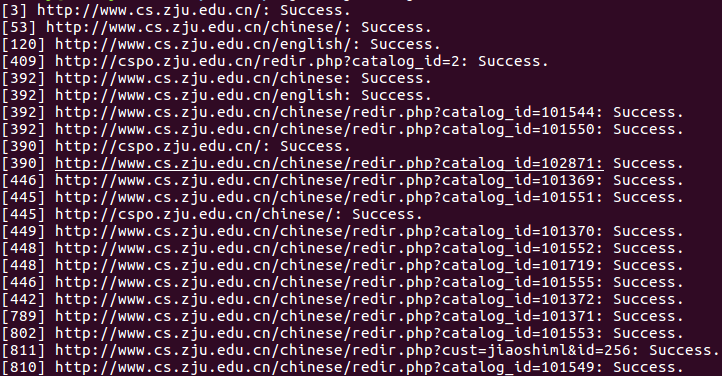
\includegraphics[scale=0.5]{pictures/0.png}
\caption{爬虫}
\label{fig:crawlShot}
\end{figure}
\autoref{fig:search1}是第一次搜索的截屏,搜索内容为我的名字``余锦成''。可以看到完全
匹配搜索结果靠前,并且命中的关键字有标注。\par
\begin{figure}[htbp]
\centering
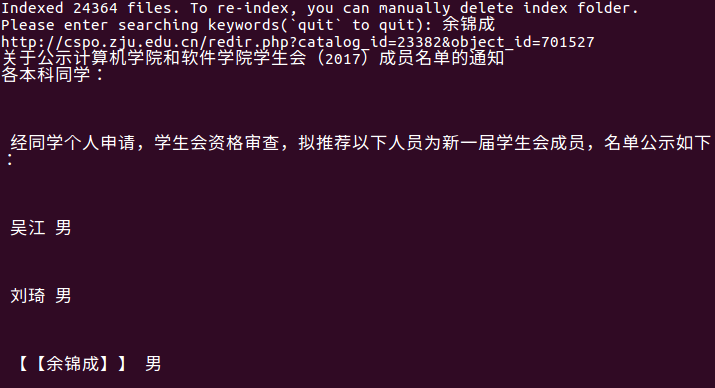
\includegraphics[scale=0.5]{pictures/1.png}
\caption{搜索}
\label{fig:search1}
\end{figure}
\autoref{fig:search2}是翻页搜索截图。这时候可以看到页码增加了,并且内容也发生了改变。\par
\begin{figure}[htbp]
\centering
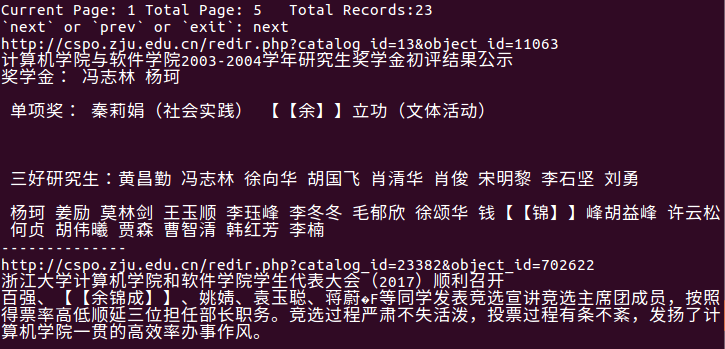
\includegraphics[scale=0.5]{pictures/2.png}
\caption{翻页}
\label{fig:search2}
\end{figure}
\autoref{fig:search3}是重新搜索截图。我们退出上次搜索结果,然后输入新的关键字,这时候又会
出现新的页面的内容。\par
\begin{figure}[htbp]
\centering
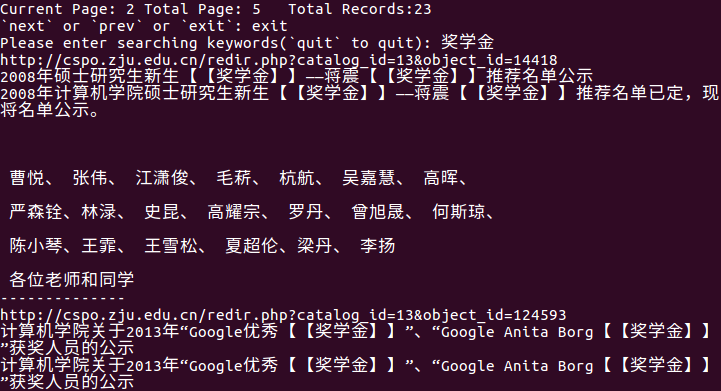
\includegraphics[scale=0.5]{pictures/3.png}
\caption{重新搜索}
\label{fig:search3}
\end{figure}
\section{总结}
这次作业综合性比较强。这次实验我们主要学习如何调用
第三方库实现我们的项目,并且阅读其文档,并组装不同
第三方库实现我们的需求。\par
除此之外,本次实验还让我们体会到Java接口、类设计的技巧,从第三方库
的实现方式真切体会,到项目中我们自己实现等。正如本次实验中,我的爬虫类
调用的实际是接口,并没有规定具体使用什么第三方库。因此,我的爬虫类在不同
环境需求下有复用性。我们可以通过实现另外一个正文提取器可以来抓取不同的网站;
可以通过修改搜索引擎类采用其他搜索引擎类。通过子类化爬虫类可以实现不同
网络获取方式, 比如我们可以改用socket来爬虫。\par
总而言之,本次实验是我对Java这门语言有了更深刻的理解,对面向接口编程
有了更深刻的实践,为我以后学习和实验打下了基础。
\end{document}
